\documentclass[11pt,openany,oneside]{article}

\usepackage{makeidx}
\usepackage{latexsym}

\usepackage[latin1]{inputenc}
\usepackage[portuguese]{babel}
\usepackage[T1]{fontenc}
\usepackage{amsmath}
\usepackage{amsfonts}


%para criar o espacamento usual no primeiro paragrafo
\usepackage{indentfirst}

%package para fazer figuras a e b automaticamente
\usepackage{subfigure}
\usepackage[pdftex]{graphicx}

% para criar os links no texto quando cita equacoes, figuras, referencias, secoes, etc...
\usepackage{hyperref}

% para colorir os links criados anteriormente
\hypersetup{ colorlinks,
linkcolor=blue,
filecolor=darkgreen,
urlcolor=blue,
citecolor=blue }
\usepackage{graphicx,color}

\usepackage{amssymb}
\usepackage{amsthm}

% este define o espacamento entre as linhas
% para referencia, 1.5 'e um espacamento grande, utilizado na minha tese de doutorado
\renewcommand*{\baselinestretch}{1.2}

%comando para colocar vetor linha
%deve ser usado com o comando \vec{p}+\pvec{p}'=\pvec{p}''
\newcommand{\pvec}[1]{\vec{#1}\mkern2mu\vphantom{#1}}


%opcao 2 para acertar as margens
\usepackage{geometry}
 \geometry{
 a4paper,
 total={210mm,297mm},
 left=20mm,
 right=20mm,
 top=20mm,
 bottom=20mm,
 }  % o valor padrao das margens right, left, top e bottom e de 20 mm

% para incluir arquivos pdf, usando o comando \includepdf
\usepackage{pdfpages}

%\pagenumbering{gobble} % remove o numero da pagina

%alinhar o texto
%\usepackage[document]{ragged2e}

%define as palavras que vao no cabecalho, mais sofisticado que o anterior
\usepackage{fancyhdr}
\pagestyle{fancy}
\fancyhf{}
%\rhead{Se��o \thesection }
\rhead{\leftmark} %\righmark = current section, and %\leftmark is current chapter
\lhead{Paulo Freitas Gomes. UFG - Jata�.}
\rfoot{\thepage}


%macros para gerar o r cursivo do griffiths
\def\rcurs{{\mbox{$\resizebox{.09in}{.08in}{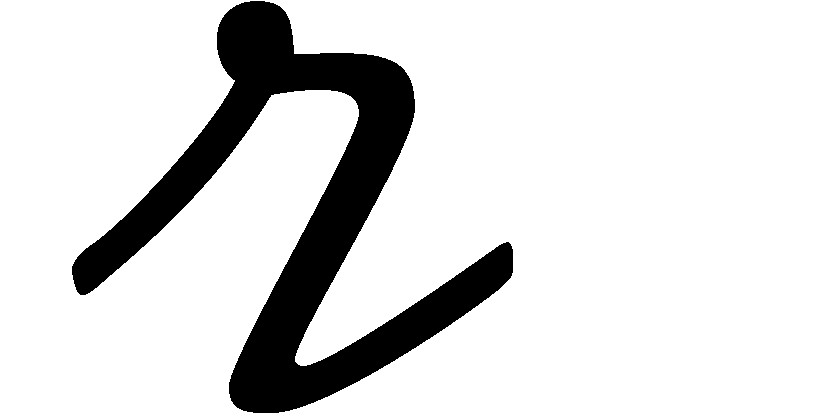
\includegraphics{ScriptR}}$}}}
\def\brcurs{{\mbox{$\resizebox{.09in}{.08in}{
\includegraphics{BoldR}}$}}}
\def\hrcurs{{\mbox{$\hat \brcurs$}}}


\begin{document}



\subsection*{Jata�, 03/02/16. Physics. UFG - Jata�.}

\subsection*{Exam 3. Eletromagnetism. Prof. Paulo Freitas Gomes.}

\vspace{0.2 in}
\noindent
Name: \noindent\rule{11cm}{0.5pt} 

\vspace{0.1 in}

\noindent
\textbf{1)} Suppose an electric and magnetic fields defined as
\begin{equation}
{\color{blue}\vec{E}(\vec{r},t) = - \dfrac{1}{4\pi \epsilon_0} \dfrac{q}{r^2} H(vt - r) \hat{r}, \qquad \vec{B}(\vec{r},t) = 0} \label{campos}
\end{equation}
where the Heaviside function is
\begin{equation}
{\color{blue}H (x) = \left\{
\begin{array}{rl}
 0 & \text{se  } x < 0  \\
\\
 1  & \text{se  } x > 0
\end{array} 
\right.} \nonumber
\end{equation}
\textbf{a)} Show that these fields satisfy the Maxwell equations. \textbf{b)} Calculate the charge $\rho$ and current $\vec{J}$ densities. \textbf{c)} Which physical situation can create such fields?


\vspace{0.1 in}
\noindent
\textbf{2) a)} A toroid has a rectangular cross section with a current $I$, $N$ tighly wound turns, inner radius $a$, outer radius $a+w$ and height $h$. Show that its magnetic field is:
\begin{equation}
{\color{blue}\vec{B} (\vec{r}) = \left\{
\begin{array}{rl}
 \dfrac{\mu_0 N I}{2\pi s} \hat{\phi} & \text{inside the toroid}  \\
\\
 0  & \text{outside the toroid  }
\end{array} 
\right.} \nonumber
\end{equation}
\textbf{b)} Now the current is increasing at a non-constant rate $dI/dt = kI$. If $w$ and $h$ are both much lower than $a$, find the electric field at a point $z$ above the center of the toroid.


\vspace{0.1 in}
\noindent
\textbf{3)} Suppose a magnetic monopole charge $q_m$ passes through a resistanceless loope of wire with self-inductance $L$. \textbf{a)} What current is induced in the loop? \textbf{b)} This is one of the methods used
to experimentally search for magnetic monopoles, see for example B. Cabrera, \textit{Phys. Rev. Lett.} \textbf{48}, 1378 (1982). From this Ref. would you say the magnetic monopole was observed? Why?


\vspace{0.1 in}
\noindent
\textbf{4)} There are many methods to solve differential equations (DE). One of them is to rewrite them in a simpler form. For example, the Maxwell equations are 4 first-order DE. \textbf{a)} Show that these equations can be written as these 2 second-order DE:
\begin{equation}
{\color{blue}\nabla^2 \vec{E} = \mu_0 \epsilon_0 \dfrac{\partial^2 \vec{E} }{\partial t^2}}, \qquad {\color{blue}\nabla^2 \vec{B} = \mu_0 \epsilon_0 \dfrac{\partial^2 \vec{B} }{\partial t^2}} \nonumber
\end{equation}
\textbf{b)} What is the meaning of the fact that both $\vec{E}$ and $\vec{B}$ satisfy the wave equation?

\vspace{0.2 in}

\begin{flushright}
\begin{small}
\textit{ ... if you're willing to go through all the battling to get where you want to be, who's got the right to stop you? Maybe you got something you never finished, something you really want to do, something you never said to anyone, and you're told no, even after you paid your dues? Who's got the right to tell you no, who? Nobody! It's your right to listen to your gut, because you have the right to be where you want to be and do whatever you want to do!
}  
\textbf{Rocky Balboa}
\end{small}
\end{flushright}


\newpage

\section*{{\color{red}Gabarito}}

\noindent
{\color{red}\textbf{1a)} 1.5 point.} The Maxwell equations are:
{\color{blue}
\begin{eqnarray}
\vec{\nabla} \cdot \vec{E} &=& \dfrac{\rho}{\epsilon_0} \label{leidegauss} \\
\vec{\nabla} \times \vec{E} &=& -\dfrac{\partial \vec{B}}{\partial t} \label{leidefaraday} \\
\vec{\nabla} \cdot \vec{B} &=& 0 \label{wiwuiwuwuwu} \\
\vec{\nabla} \times \vec{B} &=& \mu_0 \vec{J}+ \mu_0 \epsilon_0 \dfrac{\partial \vec{E}}{\partial t}  \label{leiademperemaxwell}
\end{eqnarray}}
Using $\vec{\nabla} \cdot (f\vec{A}) = f\vec{\nabla} \cdot \vec{A} + \vec{A} \cdot \vec{\nabla}f$, the divergent of the electric field from Eq. \ref{campos} is:
{\color{blue}\begin{eqnarray}
\vec{\nabla} \cdot \vec{E} &=& - \dfrac{q}{4\pi \epsilon_0} \vec{\nabla} \cdot \left[    \dfrac{\hat{r}}{r^2} H(vt - r) \right]  = - \dfrac{q}{4\pi \epsilon_0} H(vt - r) \vec{\nabla} \cdot \dfrac{\hat{r}}{r^2} - \dfrac{q}{4\pi \epsilon_0} \dfrac{\hat{r}}{r^2} \vec{\nabla} \cdot H(vt - r)  \nonumber  \\ 
&=&  -\dfrac{q}{\epsilon_0} \delta^3 (\vec{r}) H(vt - r) - \dfrac{q}{4\pi \epsilon_0} \dfrac{\hat{r} \cdot \hat{r}}{r^2} \dfrac{\partial }{\partial r} H(vt - r)  \nonumber
\end{eqnarray}}
In the last equation I used $\vec{\nabla} \cdot \dfrac{\hat{r}}{r^2} = 4 \pi \delta^3 (\vec{r})$. From the properties of the Dirac delta function we have:
{\color{blue}
\begin{eqnarray}
\delta^3 (\vec{r}) H(vt - r) &=& \delta^3 (\vec{r}) H(t) \nonumber \\
\dfrac{\partial }{\partial r} H(vt - r)  &=&  - \delta (vt - r) \nonumber
\end{eqnarray}}
Thus, using these results, the divergent of the electric field becomes:
\begin{equation}
{\color{blue}\vec{\nabla} \cdot \vec{E} = \dfrac{q}{4\pi \epsilon_0 r^2} \delta (vt - r) - \dfrac{q}{\epsilon_0 }\delta^3 (\vec{r}) H(t)} \label{sksjwjhwkwk}
\end{equation}
So, I define the charge density as:
\begin{equation}
{\color{blue}\rho = \dfrac{q}{4\pi r^2} \delta (vt - r) - q\delta^3 (\vec{r}) H(t) }\label{densidadecarga}
\end{equation}
With this in mind, the Eq. \ref{sksjwjhwkwk} can be written as:
\begin{equation}
{\color{blue}\vec{\nabla} \cdot {E} = \dfrac{\rho}{\epsilon_0}} \nonumber
\end{equation}
which is exactly the Gauss Law.

The absence of magnetic monopoles (Eq. \ref{wiwuiwuwuwu}) is clearly satisfied, once the divergence of zero is also zero. In the same way its temporal derivative is also zero:
\begin{equation}
{\color{blue}\dfrac{\partial \vec{B}}{\partial t} = 0} \label{derivadatemporalB}
\end{equation}
The curl of the electric field is also zero:
{\color{blue}\begin{eqnarray}
\vec{\nabla} \times \vec{E} &=& \dfrac{1}{r\sin \theta} \left[ \dfrac{\partial }{\partial \theta} (E_{\phi} \sin \theta) - \dfrac{\partial E_{\theta} }{\partial \phi} \right] \hat{r} + \dfrac{1}{r} \left[ \dfrac{1}{\sin \theta} \dfrac{\partial E_r}{\partial \phi} - \dfrac{\partial }{\partial r}  (rE_{\phi}) \right] \hat{\theta} + \dfrac{1}{r} \left[ \dfrac{\partial }{\partial r} (rE_{\theta}) - \dfrac{\partial E_r }{\partial \theta}   \right] \hat{\phi} \nonumber \\
&=& \dfrac{1}{r}  \dfrac{1}{\sin \theta} \dfrac{\partial E_r}{\partial \phi} \hat{\theta} - \dfrac{1}{r}\dfrac{\partial E_r }{\partial \theta} \hat{\phi} = 0 \label{sksjwuwjsu}
\end{eqnarray}}
given that $E_{\theta} = E_{\phi} = 0$ and $E_r$ only depends on $r$. From the Eqs. \ref{derivadatemporalB} and \ref{sksjwuwjsu} we have that Faraday's Law (Eq. \ref{leidefaraday}) is also satisfied.  

Now there is only Amp�re Maxwell Law missing. Clearly the curl of the magnetic field is zero: $\vec{\nabla} \times \vec{B}=0$. If we define the volumetric current density as
\begin{equation}
{\color{blue}\vec{J} = -\epsilon_0 \dfrac{\partial \vec{E}}{\partial t} = \dfrac{q}{4\pi r^2} \hat{r}\dfrac{\partial }{\partial t} H(vt - r)  =   \dfrac{q}{4\pi r^2} \hat{r} v\delta (vt - r)} \label{densiddeJ}
\end{equation}
we will have
\begin{equation}
{\color{blue}\mu_0 \vec{J} + \mu_0 \epsilon_0 \dfrac{\partial \vec{E}}{\partial t} = 0 = \vec{\nabla} \times \vec{B}} \nonumber
\end{equation}
which is exactly the Amp�re Maxwell Law (Eq. \ref{leiademperemaxwell}).

It may look artificial using arbitrary definitions of $\rho$ and $\vec{J}$ to make the $\vec{E}$ from Eq. \ref{campos} satisfy Maxwell Equations. The important point is to make sure that there is a physical situation which generates such $\rho$ and $\vec{J}$.
 
 
\noindent
{\color{red}\textbf{1b)} 0.5 point.} The carge density $\rho$ and current density $\vec{J}$ are defined by the Eqs. \ref{densidadecarga} e \ref{densiddeJ}.

\noindent
{\color{red}\textbf{1c)} 0.5 point.} It is the field of a point charge $-q$ at the origin and an expanding spherical shell of radius $vt$, outside this shell the field is zero. The shell carries a charge of $+q$. The charge $-q$ does not contribute to the current $\vec{J}$, although for the spherical shell we have $\vec{J} = \rho \vec{v}$.


 \vspace{0.1 in}
 
\begin{center}
\noindent\rule{9cm}{0.4pt}
\end{center}

\begin{figure}[!h]
\centering
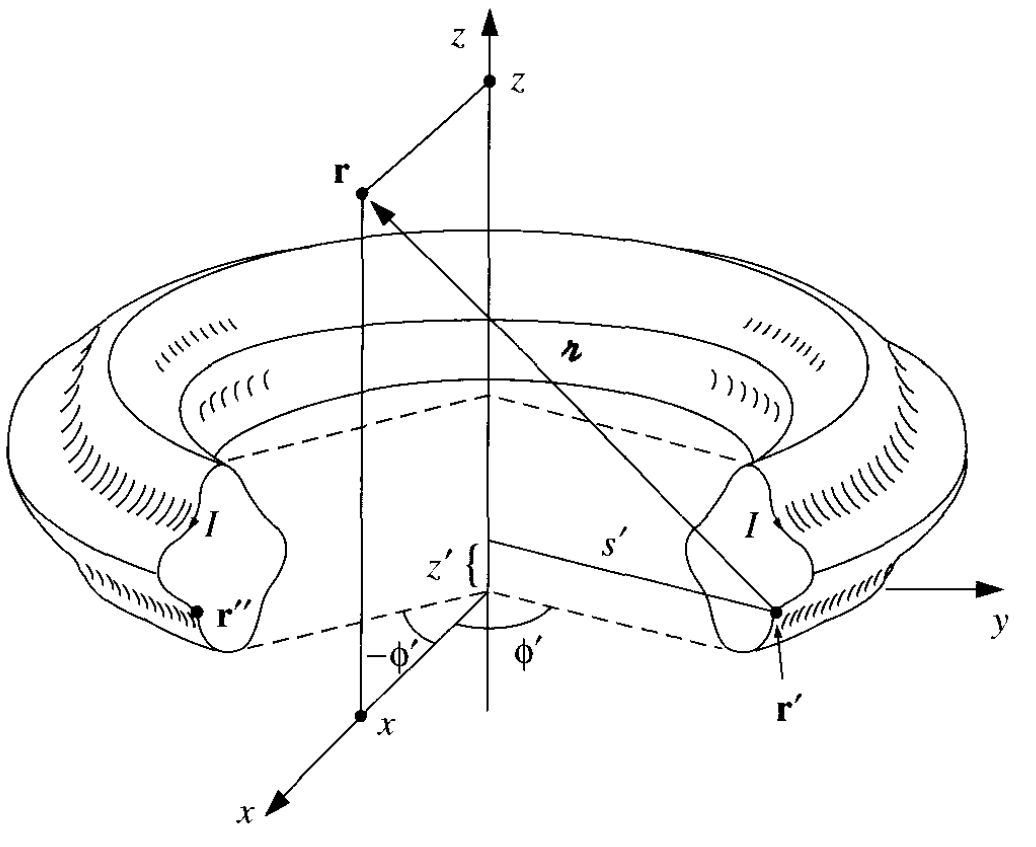
\includegraphics[width=4.0 in]{figuras/toroide_geometria.png}
\caption{Geometry for the toroid coil of problem 2.}
\label{toroide}
\end{figure}



\noindent
{\color{red}\textbf{2a)} 1 point} From Biot Savart's Law, the magnetic field is:
\begin{equation}
{\color{blue}d \vec{B} = \dfrac{\mu_0 }{4\pi} \dfrac{ \vec{I} \times \vec{\rcurs}}{r^3} dl' }
\end{equation}
We must choose an arbitrary position to calculate the field. Without lost of generality, we choose to put it in the $xz$ plane so that $\vec{r} = (x,0,z)$ (see figure \ref{toroide}). In this way the position of integration and separation vector are:
{\color{blue}\begin{eqnarray}
\vec{r}' &=& (s' \cos \phi', s' \sin \phi', z')  \nonumber \\ 
\vec{\rcurs}  &=& \vec{r} - \vec{r}' = (x - s' \cos \phi', s' \sin \phi', z - z')  \nonumber
\end{eqnarray}} 
The current has no $\phi$ componente so:
\begin{equation}
{\color{blue}\vec{I} = I_s \hat{s} + I_z \hat{z} = (I_s \cos \phi', I_s \sin \phi', I_z ) }
\end{equation}
The cross product will be:
{\color{blue}\begin{eqnarray}
\vec{I} \times \vec{\rcurs} &=& (I_s \cos \phi', I_s \sin \phi', I_z ) \times (x - s' \cos \phi', s' \sin \phi', z - z') \nonumber \\
&=& \left[ (I_s(z-z')+s'I_z)\sin \phi' \right] \hat{i} + \left[ I_z (x - s' \cos \phi' ) - I_s (z-z') \cos \phi' \right] \hat{j} - I_s x \sin \phi' \hat{k}   \label{qwerasdf}
\end{eqnarray}}
However there is always a symmetrically situated current element at $\vec{r}''$ e $\pvec{r}$ with the same $s'$, the same $\rcurs$, the same $dl'$, the same $I_s$ and $I_z$, but with negative $\phi'$. As $\sin \phi = - \sin (-\phi)$, the $\hat{i}$ and $\hat{k}$ contributions in Eq. \ref{qwerasdf} cancel out leaving only the $\hat{j}$ term. So the magnetic field at a point $\vec{r}$ is in the $y$ direction. For an arbitrary point, it will point in the $\hat{\phi}$ direction.

Now we can state that the field is circumferential and apply Amp�re's Law to calculate its magnitude:
\begin{equation}
{\color{blue}\oint_C \vec{B} \cdot d\vec{l} = \mu_0 I_c} \label{amperelawintegral}
\end{equation}
where $I_c$ is the total current enclosed by the amperian C. As the field is on $\hat{\phi}$ direction, I choose as amperian a circle in the $xy$ plane inside the toroid. The magnitude of $\vec{B}$ will be constante and it is parallel to $d\vec{l}$:
{\color{blue}\begin{equation}
\int_C \vec{B} \cdot d\vec{l} = \int_C B dl = B \int_C dl = 2\pi s B = \mu_0 I_c
\end{equation}}
So $B = \dfrac{\mu_0 I_c}{2\pi s}$ inside the coil and zero outside. The total current is $I_c = NI$, thus:
\begin{equation}
{\color{blue}\vec{B} (\vec{r}) = \left\{
\begin{array}{rl}
 \dfrac{\mu_0 N I}{2\pi s} \hat{\phi} & \text{inside the toroid}  \\
\\
 0  & \text{outside the toroid  }
\end{array} 
\right.} \nonumber
\end{equation}


\noindent
{\color{red}\textbf{2b)} 1.5 point} The differential equation $dI/dt = f(I,t)$ (for any $f(I,t)$) specify the variation $I(t)$. This creates a time varying magnetic field which in turns can create an electric field from the Faraday Law (Eq. \ref{leidefaraday}). However it is not simple to obtain one vector only knowing its curl. So we need another strategy. As there is a symmetry, we will use the Faraday Law in the integral form:
\begin{equation}
{\color{blue}\oint \vec{E} \cdot d\vec{l} = -\dfrac{d\Phi}{dt}}  \nonumber
\end{equation}
Now, take a look at Amp�re Law in integral form (Eq. \ref{amperelawintegral}): $-\dfrac{d\Phi}{dt}$ creates an electric field the same way $\mu_0 I$ creates a magnetic one. For example, a circular loop in the $xy$ plane with current $I$ and radius $a$ creates a magnetic field in the $z$ direction
\begin{equation}
{\color{blue}\vec{B}_l = \dfrac{\mu_0 I}{2} \dfrac{a^2 \hat{k}}{(a^2 + z^2)^{3/2}}} \nonumber
\end{equation}
So, a time dependent magnetic flux tangent to the circular loop will create an electric field also in the $z$ direction\footnote{The current is a scalar but it has a direction. The flux $\Phi$ is also a scalar, however we can think of its direction as the direction of the magnetic field creating the flux, which in this case is the same direction as the current from the circular loop.}. We just need to change $\mu_0I$ by $-d\Phi /dt$. Then, in analogy to the last equation, the electric field will be:
{\color{blue}\begin{equation}
\vec{E} = - \dfrac{1}{2} \dfrac{d\Phi}{dt} \dfrac{a^2 \hat{k}}{(a^2 + z^2)^{3/2}} \label{slwlekejejwwww}  
\end{equation}}
We must now calculate the magnetic flux:
\begin{equation}
{\color{blue}\Phi(t) =\int \vec{B} \cdot d\vec{a} = \dfrac{\mu_0 NI(t)}{2\pi} \int_a^{a+w} \dfrac{hds}{s} = \dfrac{\mu_0 Nh I(t)}{2\pi} \ln \left( 1+ \dfrac{w}{a} \right) \approx \dfrac{\mu_0 Nhw}{2\pi a}  I(t)} \nonumber 
\end{equation}
In the last passage we kept only the first term of the expansion of the natural logarithm
{\color{blue}\begin{equation}
\ln (1+x) = \sum_{n=1}^{\infty}  \dfrac{x^n}{n}(-1)^{n+1} = x - \dfrac{x^2}{2} + \dfrac{x^3}{3} - \dfrac{x^4}{4} + ... \approx x
\end{equation}}
which is valid when $x << 1$. Its derivative will be:
\begin{equation}
{\color{blue}\dfrac{d\Phi}{dt} = \dfrac{\mu_0 Nhw}{2\pi a}  \dfrac{dI}{dt}}  \nonumber
\end{equation}
So Eq. \ref{slwlekejejwwww} becomes:
\begin{equation}
{\color{blue}\vec{E} = - \dfrac{1}{2} \dfrac{a^2 \hat{k}}{(a^2 + z^2)^{3/2}} \dfrac{\mu_0 Nhw}{2\pi a}  \dfrac{dI}{dt} } \nonumber
\end{equation}
If we consider $dI/dt = kI$ we have $I(t) = I_0 e^{kt}$. Then:
\begin{equation}
{\color{blue}\vec{E}(t) = - \dfrac{1}{2} \dfrac{a^2 \hat{k}}{(a^2 + z^2)^{3/2}} \dfrac{\mu_0 Nhw}{2\pi a}  kI_0 e^{kt} } \nonumber
\end{equation}
It is important to leave the final answer as function of the time, and not of the current $I$.
However, if we consider $dI/dt = kt$ we have:
\begin{equation}
{\color{blue}\vec{E}(t) = - \dfrac{1}{2} \dfrac{a^2 \hat{k}}{(a^2 + z^2)^{3/2}} \dfrac{\mu_0 Nhw}{2\pi a}  kt}  \nonumber
\end{equation}

 \vspace{0.1 in}
 
\begin{center}
\noindent\rule{9cm}{0.4pt}
\end{center}


\noindent
{\color{red}\textbf{3a)} 2 points} In case there exist a magnetic charge $q_m$, we can define a magnetic charge current $I_m$ and density current $\vec{J}_m$ as:
\begin{equation}
{\color{blue}I_m = \dfrac{dQ_m}{dt} = \int_S \vec{J}_m \cdot d\vec{a} } \nonumber
\end{equation}
In order to calculate $I_m$, we need one equation which involves it. The only possible equation is a generalized Faradays Law:
\begin{equation}
{\color{blue}\vec{\nabla} \times \vec{E} = -\mu_0 \vec{J}_m -\dfrac{\partial \vec{B}}{\partial t} } \nonumber
\end{equation}
which follows the analogy with Amp�re Maxwell Law. As we suppose the magnetic charge passes through the loop, let's integrate the last equation in the enclosed surface of the loop:
\begin{equation}
{\color{blue} \int (\vec{\nabla} \times \vec{E}) \cdot d\vec{a} = -\mu_0  \int \vec{J}_m \cdot d\vec{a}  -\dfrac{\partial }{\partial t} \int \vec{B} \cdot d\vec{a}} \label{sllwkwjwkjww}
\end{equation}
Using Stokes Theorem, the electromotive force is:
\begin{equation}
{\color{blue}\int (\vec{\nabla} \times \vec{E}) \cdot d\vec{a} = \int \vec{E} \cdot d\vec{l} = \varepsilon } \nonumber
\end{equation}
Eq. \ref{sllwkwjwkjww} can be written as:
\begin{equation}
{\color{blue}\varepsilon = -\mu_0 I_m - \dfrac{d \Phi_m}{dt}} \nonumber
\end{equation}
where $\Phi_m$ is the magnetic flux through the surface. Using the definition of indutance $\varepsilon = -LdI/dt$, we have:
\begin{equation}
{\color{blue}\dfrac{dI}{dt} = \dfrac{\mu_0 I_m}{L} + \dfrac{1}{L} \dfrac{d \Phi_m}{dt}} \nonumber
\end{equation}
If we take an approximate average in time of the last equation in a time $\Delta t$ we have:
\begin{equation}
{\color{blue}I = \dfrac{\mu_0 \Delta Q_m}{L} + \dfrac{\Delta \Phi_m}{L}} \nonumber
\end{equation}
So, if a magnetic charge $q_m$ passes through the loop the induce current will be:
\begin{equation}
{\color{blue}I(q_m) = \dfrac{\mu_0 q_m}{L}  } \nonumber
\end{equation}
We have $\Delta \Phi_m = 0$ because the flux is both zero when the charge $q_m$ is far away before entering the loop and far away after passing through the it. 


\noindent
{\color{red}\textbf{3b)} 0.5 point} The mentioned article reports results from a superconductor detector for magnetic moving charges. As we saw in the previous item, a magnetic charge can be detected using a loop detector. Indeed, as described in the paper, they use the generalized Faraday Law, and considered relativistic effects, to express the measured current as function of the magnetic charge $q_m = \varphi_0 / (2\pi)$:
\begin{equation}
{\color{blue}I(t) = \dfrac{\varphi_0}{L} \left[ 1+ \dfrac{\gamma v t}{\sqrt{(\gamma v t)^2 + b^2}} \right] }
\end{equation}
The detector is made of a superconductor material to increase the sensibility for the current. From March 11st 1982, data have been recorded for a total of 151 days. Typical results, with no relevant detection is shown in Figure \ref{results_cabrera}a). However, a single, large and rare event was recorded and the result is shown in the graph of Figure \ref{results_cabrera}b). Indeed, we can see a variation up to $7\varphi_0$. Many technical and experimental effects are extensively discussed in the paper in how they tried to avoid its influences. Even though, the author can not argue that the recorded event (and others) are result from a magnetic charge.


 \begin{figure}
 \centering
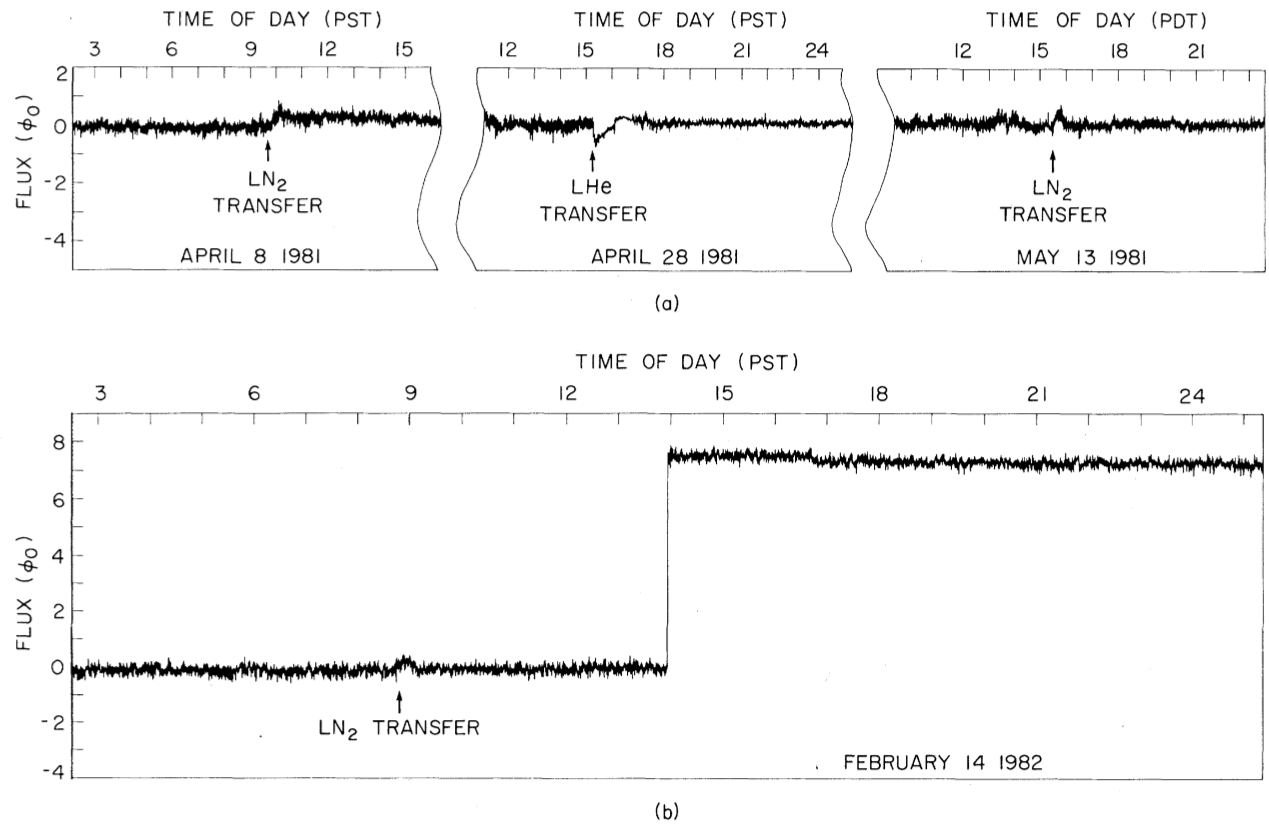
\includegraphics[width=5.0 in]{figuras/results_cabrera.png}
\caption{Corrente em fun��o da tens�o. a) Typical results. b) Single rare event recorded. Figure from PRL \textbf{48} 1378 (1982).}
\label{results_cabrera}
\end{figure}

 \vspace{0.1 in}
 
\begin{center}
\noindent\rule{9cm}{0.4pt}
\end{center}


\noindent
{\color{red}\textbf{4a)} 1.5 point} Let's consider the vacuum where $\rho = \vec{J} = 0$. The Gauss and Amp�re Maxwell Laws become:
{\color{blue}\begin{equation}
 \vec{\nabla} \cdot \vec{E} = 0, \qquad   \vec{\nabla} \times \vec{B} = \mu_0 \epsilon_0 \dfrac{\partial \vec{E}}{\partial t}  \label{amperemaxwellmono}
\end{equation}}
The idea to obtain the wave equation for the fields is to calculate the curl of the curl of them in two different ways. In the first way we will use the following property:
\begin{equation}
{\color{blue}\vec{A} \times (\vec{B} \times \vec{C})=\vec{B} (\vec{A} \cdot \vec{C})- \vec{C} (\vec{A} \cdot \vec{B})} \nonumber
\end{equation}
For the electric field:
\begin{equation}
{\color{blue}\vec{\nabla} \times (\vec{\nabla} \times \vec{E}) = \vec{\nabla} (\vec{\nabla} \cdot \vec{E})-\nabla^2 \vec{E} = -\nabla^2 \vec{E}} \label{eqnablaE}
 \end{equation}
where we used $\vec{\nabla} \cdot \vec{E}=0$. The second way is to calculate the curl of the Faraday's Law:
\begin{equation}
{\color{blue}\vec{\nabla} \times (\vec{\nabla} \times \vec{E}) = -\dfrac{\partial }{\partial t} \vec{\nabla} \times \vec{B} = -\dfrac{\partial }{\partial t} \left( \mu_0 \varepsilon_0 \dfrac{\partial }{\partial t} \vec{E}\right)  = - \mu_0 \varepsilon_0 \dfrac{\partial^2 \vec{E}}{\partial t^2}}  \label{eqnablaE2}
 \end{equation} 
 From Eqs. \ref{eqnablaE} e eq \ref{eqnablaE2} we have:
\begin{equation}
{\color{blue}\nabla^2 \vec{E} = \dfrac{1}{c^2}\dfrac{\partial^2 \vec{E}}{\partial t^2}} \nonumber
\end{equation}
where $c=\dfrac{1}{\sqrt{\varepsilon_0 \mu_0}}$ is the velocity of the wave. The case of magnetic field is the same:
{\color{blue}\begin{eqnarray}
\vec{\nabla} \times (\vec{\nabla} \times \vec{B}) &=& \vec{\nabla} (\vec{\nabla} \cdot \vec{B})-\nabla^2 \vec{B} = -\nabla^2 \vec{B} \nonumber \\
&=&  \vec{\nabla} \times \left( \mu_0 \epsilon_0 \dfrac{\partial \vec{E}}{\partial t} \right) =   \mu_0 \epsilon_0 \dfrac{\partial }{\partial t} \left( \vec{\nabla} \times \vec{E} \right) = - \mu_0 \epsilon_0 \dfrac{\partial^2 \vec{B} }{\partial t^2} 
 \end{eqnarray}}
 Thus:
\begin{equation}
{\color{blue}\nabla^2 \vec{B} = \dfrac{1}{c^2}\dfrac{\partial^2 \vec{B}}{\partial t^2}} \nonumber
\end{equation}
 
{\color{red}\textbf{4b)} 1 point} The wave equation predicts the wave behaviour, for example the mechanical waves: sound, waves in water and in strings. When Maxwell wrote his equations, it was not know that magnetic and electric field could be waves. So, the first evidence of this was the theoretical work of Maxwell, showing that $\vec{E}$ and $\vec{B}$ satisfy the wave equation, later called electromagnetic wave. After this, researchers started to look for experimental evidences of this fact. And the first one was the measurement of the speed of radio waves: the result was exactly $c =\dfrac{1}{\sqrt{\varepsilon_0 \mu_0}}$, as expected. This is an evidence that radio waves are electromagnetical ones. Then, light had its velocity measured: exactly $c$. Then, microwaves, X-rays, showing that all this waves form the so called electromagnetic spectrum.


\end{document}



